\chapter{Selection of Language Model} \label{chapter:analysis}
This chapter will cover the first two research questions about existing BERT models and how well they fit to the semiconductor domain. In this way we were able to find a suitable entrypoint for training our FA-BERT model.

\section{Overview of BERT based Models}

\subsection{RoBERTa}

\subsection{Med-BERT}

\subsection{SciBERT}
The development of BERT was a milestone in Natural language processing. Since the vocabulary of BERT is restricted, the application of the model in some domains does not lead to a satisfactory performance. To achieve this goal in different scientific fields, the model of BERT got adapted to SciBERT. The SciBERT model follows the same architecture as BERT but is instead pre-trained on scientific text. The corpus consists of 1,14M papers derived from \textit{Google Scholar}, 18\% papers from the computer science domain and 82\% from the broad biomedical domain. The authors used the full text of the papers instead of only the abstracts. The average paper length is 154 sentences which results in 2.769 tokens. The final corpus size has 3.17B tokens, similar to the 3.3B tokens on which BERT was trained \cite{Beltagy}. \newline

The S2ORC-SciBERT is a SciBERT model which was further trained on the S2ORC dataset presented above. It got published simultaneously with the dataset itself from the same developers. Compared to SciBERT it has a wider corpus including 20 different domains like Computer Science, Mathematical Science and Engineering which could be beneficial for the FA domain. However it was also trained on Medical and Biology data which again could be a drawback for the model as with SciBERT.

\subsection{S2ORC-SciBERT}

\section{Choosing the Model Entrypoint}
Since BERT models studied in this paper were trained on different text corpora, their tokenizers might provide different coverage of important terms used in the FA domain, such as the ones stored in FA ontology. To determine the coverage, we first analyze the tokenization of the ontology keywords with the three language models: traditional BERT, SciBERT and S2ORC-SciBERT. With this analysis it was possible to gain a first impression about the vocabulary of the models and how well they fit to the electrical domain. \newline
The models got downloaded from the website \alert{Huggingface} and can be load into the notebook as follows:
\begin{minted}{python}
	model = BertModel.from_pretrained("/path/to/model/")
	tokenizer = BertTokenizer(vocab_file = '../path/to/tokeizer/vocab.txt')
\end{minted}

To receive the keywords, we executed an existing function provided from our supervisor Christian Burmer. It executes a script with a request to the SparQL Database receiving the ontology keywords in a list. This keywords also occur in the reports as indicators for the content. \newline
After receiving the keywords from the ontology and having a deeper look at them, we found some misspellings like in the word \textit{flasover}, which misses a h to become \textit{flashover}. These typos could confuse the models and lead to some mistokenization. To prevent this, we will first run some spell checking and correction methods on the keywords before further processing it. Therefore we tried different packages like the \textit{Pyspellchecker} or \textit{SymSpellPy} which are based on the \textit\alert{{Peter Novig's method}}. As both of the two packages did not work, we skimmed the keywords manually and corrected misspellings. \newline
With the correct spelled keywords we started the experiment of tokenizing them with the three different BERT models. The code for tokenization was the same for every model:
\begin{minted}{python}
	# Run tokenizer.
	tokenized_word = s2orc_scibert_tokenizer.tokenize(word)
	
	#differentiate good and badly tokenized words
	if len(tokenized_word) == 2:
		good_tokenized_words_s2orc += 1
		good_words.extend(tokenized_word) 
	elif len(tokenized_word_c) > 2:
		badly_tokenized_words_s2orc += 1
		bad_words.extend(tokenized_word)
\end{minted}

We created a loop which hands every word over to the tokenizers and also analyzes if the resulting word is included in the models vocabulary or not. A word which is already in the vocabulary will not be divided into subtokens and so consists of only one token. If it is not included in the vocabulary, we determined if the word was good or badly tokenized. A word got considered as badly tokenized if it was split in more than two tokens. Otherwise the tokenization got considered as good. At the end of the execution, we created a dataframe depicting how the individual words got splitted into tokens. An example of the dataframe is depicted in Figure \ref{fig:goodAndBad}. Here the keyword "lifted clip" would get considered as badly tokenized word and the keyword "requestor" as good.

\begin{figure}[H]
	\centering
	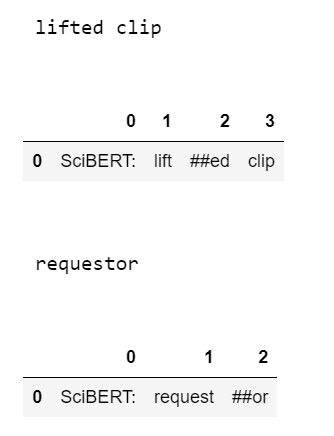
\includegraphics[width=0.3\textwidth]{figures/example_good_bad.PNG}
	\caption{Example of tokenization with SciBERT}
	\label{fig:goodAndBad}
\end{figure}


Next we analyzed the word stems of the failure analysis reports and again examined the tokenization of the words with the language models. We did not analyze the word stems of the whole reports, but only the word stems of the most frequently used words. To obtain the frequency distribution and the word stems of the reports, we used the NLTK (Natural Language Toolkit) library. It includes the so called \textit{SnowballStemmer}, because according to the documentation, this stemmer works better for English text. Stemmers remove morphological affixes from words, leaving only the word stem. To run the tokenization experiment, we also had to lower case the word stems and transform plural words into singles. The code can be seen in the code below. For the tokenization itself, the same code has been used as already explained above.

\begin{minted}{python}
	#create a new stemmer
	stemmer = SnowballStemmer("english")
	
	#test the stammer on pluralized words
	most_common_stems = nltk.word_tokenize(str(most_common))
	singles = [stemmer.stem(plural) for plural in most_common_stems]
	word_stems = set(singles)
	print(' '.join(singles))
\end{minted}

As a result of the tokenization of the keywords it can be seen that SciBERT and S2ORC-SciBERt both perform better on the keywords as the traditional BERT model. Both models contain a few more keywords in their vocabulary than the BERT model. The resulting statistic can be seen in Figure \ref{fig:comparison}. We expected this result because the training data of these two models fits better to our electrical domain than the data BERT was trained with which is more widespread.


\begin{figure}[H]
	\centering
	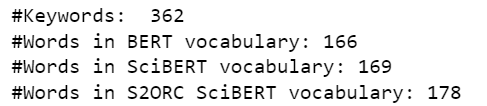
\includegraphics[width=0.5\textwidth]{figures/keyword_comparison.PNG}
	\caption{Comparison of the performance of the three models on the keywords}
	\label{fig:comparison}
\end{figure}


For the tokenization of the FA reports and their word stems we assumed to see at least a slight difference between SciBERT and S2ORC-SciBERT but without fine-tuning the models it is not possible to determine a better model which can be seen on the results of the tokenization analysis in Figure \ref{fig:stemming_performance}.


\begin{figure}[H]
	\centering
	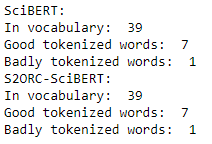
\includegraphics[width=0.3\textwidth]{figures/wordstems_comparison.PNG}
	\caption{Comparison of the performance on the word stems}
	\label{fig:stemming_performance}
\end{figure}

\alert{In order to finally decide between SciBERT and S2ORC-SciBERT, a further analysis was performed in which the keywords were assigned a weighting based on their occurrence frequency. This makes it possible to assign an importance to the keywords. The more often they appear in the reports, the more important it is that the model tokenizes the keywords well. Therefore, using the frequency and the number of subtokens, a weight is calculated as follows:}
\begin{align}
	n &= |t_1, t_2, ... t_n| \\
	\to w &= n \cdot sx_m
\end{align}

The resulting weights looked like the following:
\begin{minted}{python}
	[('thin', 0.002654), ('backside', 0.062375), ('metallization', 0.12209),...]
\end{minted}

After this weighting we again performed a tokenization and examined the good and badly tokenized keywords, but both models performed again very similar. SciBERT tokenized 129 keywords good, S2ORC-SciBERT 120. Because the FA reports contain out of more than only keywords, we decided to choose the S2ORC-SciBERT as an entrypoint for our further experiments. It has more electrical and physical papers in its training corpus than the original SciBERT and therefore might work better for us.